%% ==============================
\chapter{Concept}
\label{sec:concept}
%% ==============================
The problem of multi-floor navigation can generally be split up in the following six sub-problems:

\begin{enumerate}
    \item \textbf{Model the Environment}\\\
    Output: Gridmaps, locations of hierarchical connections
    \item \textbf{Hierarchy Creation}\\
    Output: Room segmentation, H-Graph
    \item \textbf{Generate Roadmaps}\\
    Output: Pre-computed paths between hierarchies
    \item \textbf{Hierarchical Planning}\\
    Output: Collision free path from start to goal
    \item \textbf{Execute with a Mobile Robot}\\\
    Output: Behavior tree for multi-floor navigation
    \item \textbf{Interact with Infrastructure}\\
    Output: Hardware interfaces, Behavior Trees
\end{enumerate}

This chapter outlines the concepts of this work for solving these problems. It also highlights the limitations of the scope of this work. The fundamental step for navigating in a multi-floor environment is to gather information about the environment and create a model that represents all relevant information for navigating in the specific buildings. At a minimum, this includes a representation of the drivable area on each floor. This can be in the form of a discretized gridmap, a 3D voxel representation as Octomap \cite{hornung_octomap_2013} or other visual markers. Within the defined coordinate system, the locations of all hierarchical connections must be marked. These could be doors between rooms, elevators between floors, or connections between buildings such as bridges or ramps. For maximum autonomy, the goal would be to autonomously generate these while exploring the entire environment. Although frameworks for autonomous exploration and mapping exist, this is beyond the scope of this work. To model the test environment in the lab and in simulation, manual gridmaps were created using \gls{slam}. The locations of elevators and connections between buildings were created manually. Only the connections at the lowest hierarchical level, which are doors between rooms, were automatically created from the provided gridmaps as part of the room segmentation.

Hierarchy creation is done in two steps. First, the model of the environment has to be split into its respective hierarchical structure, and second, an H-Graph is created that represents the hierarchical connections and holds the individual parts of the environment at its lowest level. For the segmentation of rooms from gridmaps, the marker-controlled watershed algorithm from \cite{parvati_image_2009} was used. Only the automatic hierarchy creation of rooms from gridmaps is in the scope of this work. Higher levels of hierarchy are created manually. To find the hierarchical bridge points, here: doors between rooms, the optimal locations are extracted during the segmentation process. This is inspired by the approach of \cite{ryu_hierarchical_2020}. Details on the specific implementation follow in Chapter \ref{sec:hierarchy_creation}.

Roadmap generation follows the principles outlined in the problem statement. That is, the goal is to find paths that are straight, deterministic, and predictable. The concept in this work takes this into account by generating straight paths that are mostly parallel to the walls. This is done by first rotating the gridmap to be parallel to the axis of the coordinate frame and then iteratively generating the largest free rectangle in each room. This straight path planner is called \gls{ilir}. These rectangles are then merged into a single polygon and connected to all doors to adjacent rooms. The advantages of this approach are listed below:

\begin{enumerate}
    \item Deterministic, the robot always takes the same path
    \item Straight paths that follow the walls
    \item Predictable for bystanders
    \item Reduce anxiety for passengers
    \item Avoids disturbance of public space
    \item Can be represented as a graph and searched very quickly
\end{enumerate}

The drawbacks of \gls{ilir} are that this planner does not provide optimal paths and includes sharp 90 degree turns. The rectangular corners are later smoothed by the controller of the \gls{nav_2} stack, which follows the generated path with a maximum turning angle. This pre-calculated roadmap now connects all hierarchical neighbors, such as other rooms through doors and other floors through elevators. These roadmaps form the basis for path planning in each room, and arbitrary start or end points are later connected to this graph. The graph representing the roadmap is the lowest hierarchy level in the \gls{h_graph}. Implementation details are given in Chapter \ref{sec:roadmap_generation}.

%% ==============================
\section{Hierarchical Planning}
\label{sec:hierarchical_planning_method}
%% ==============================
Once an H-Graph of the environment is created, the next problem is to solve the planning for a given pair of start and goal locations. Each may be on different floors in completely different buildings. This requires planning across multiple subgraphs. In this concept, the individual hierarchical entities, such as rooms, floors, or buildings, represent a node in the graph one hierarchy level higher. Figure \ref{fig:hierarchical_planning} shows each hierarchical level of the \gls{iras} research campus.

\begin{figure}[htb]
    \captionsetup[subfigure]{justification=centering}
    \centering
    % \begin{subfigure}{\textwidth}
    %   \centering
    %   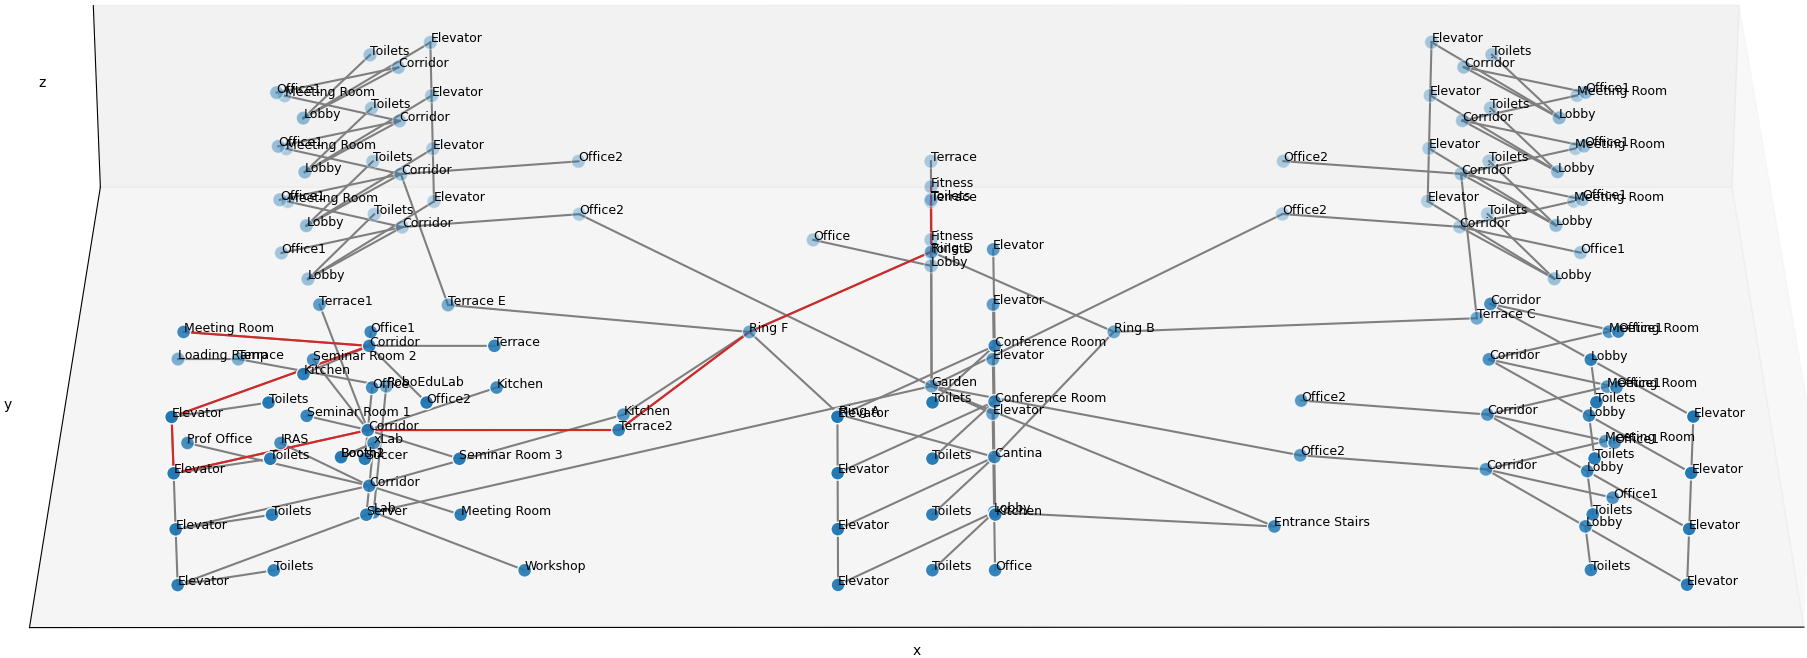
\includegraphics[width=\textwidth]{figures/40_concept/ltc_graph_complete.png}
    %   \caption{Overview graph just for visualization}
    % \end{subfigure}
    \begin{subfigure}{.4\textwidth}
      \centering
      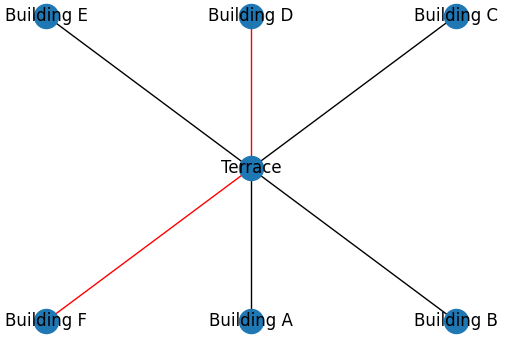
\includegraphics[width=\textwidth]{figures/40_concept/ltc_graph_campus.png}
      \caption{Graph of research campus (H4)}
    \end{subfigure}%
    \begin{subfigure}{.6\textwidth}
      \centering
      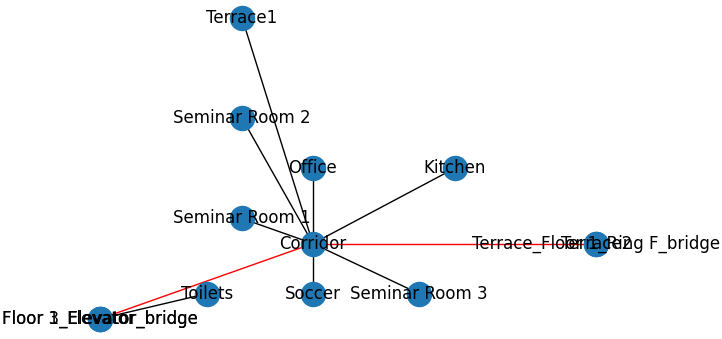
\includegraphics[width=\textwidth]{figures/40_concept/ltc_graph_floor_2.png}
      \caption{Graph of Floor 2, Building F (H2)}
    \end{subfigure}
    \begin{subfigure}{.2\textwidth}
      \centering
      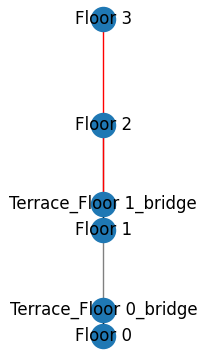
\includegraphics[width=\textwidth]{figures/40_concept/ltc_graph_building_f.png}
      \caption{Graph of Building F (H3)}
    \end{subfigure}%
    \begin{subfigure}{.8\textwidth}
      \centering
      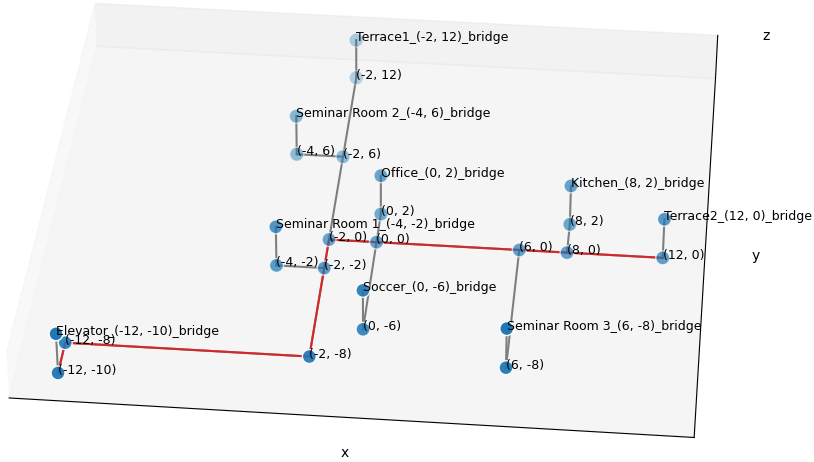
\includegraphics[width=\textwidth]{figures/40_concept/ltc_graph_corridor.png}
      \caption{Graph of Corridor on Floor F2 (H1)}
    \end{subfigure}
    \caption[Hierarchical path planning with 4 hierarchy levels]{Hierarchical planning with 4 hierarchy levels (H1 - H4) and solution path from Meeting Room to Fitness Studio (red). a) Buildings of the campus. b) Rooms of the Floor F2. c) Floors of Building F. d) Roadmap of the Corridor on the lowest hierarchy. Bridges to other adjacent hierarchies are in \(z+1\) and have no path cost.}
    \label{fig:hierarchical_planning}
\end{figure}

The advantage of this approach is a more intuitive representation, a better mapping of the corresponding gridmap to the nodes, and a smaller and less dense H-Graph. The disadvantage of this concept is a more complex hierarchical planning algorithm, because in the top-down search the absolute distances of the lower levels are not known. This results in the need to compute all possible solutions to the goal at one hierarchy level, and then to explore each node on its corresponding subgraph and compute all possible solutions in that graph as well, until the lowest hierarchy is reached. From this top-down search, multiple possible paths are reconstructed and combined at the lowest level. Finally, all feasible paths must be compared in length to select the optimal path. In comparison, Seder et al. \cite{seder_hierarchical_2011} uses the bridge points as hierarchy nodes in the graph, so all possible paths can be easily precomputed and already at the highest hierarchy level only the shortest path needs to be explored deeper. This drawback of the current concept can be addressed in two ways: First, by introducing a heuristic such as the Euclidean distance that estimates the minimum distance between nodes on a lower level and thus allows to search for the optimal path with an A* instead of a Dijsktras algorithm. The second solution would be to provide a mapping on the parent node that contains all possible combinations of connections of possible start and target nodes in the subgraph and their corresponding costs. This can be precomputed from bottom to top and then used later to efficiently search from top to bottom. Neither solution is currently implemented. This concept uses the approach of exploring all possible solutions to their maximum depth and then comparing for the shortest solution.

%% ==============================
\section{Execution with a Mobile Robot}
\label{sec:execution}
%% ==============================
To bring together all the previous concepts, a behavior tree is used to coordinate all the different subtasks. Since the goal of this work is to enable a real robot to navigate between different floors, problems 1-4 must be wrapped in ROS 2 nodes to interact with the rest of the robot's hardware and to be able to listen to commands from the Behavior Tree framework used. Chapter \ref{sec:navigation_stack} introduced the default \gls{nav_2} stack and its architecture for mobile robot navigation. This modular architecture is now extended with custom planner plugins and integrated into the simulation and the real PeTRA robot. Figure \ref{fig:concept_nav2} shows the extended architecture. 

\begin{figure}[h]
    \centering
    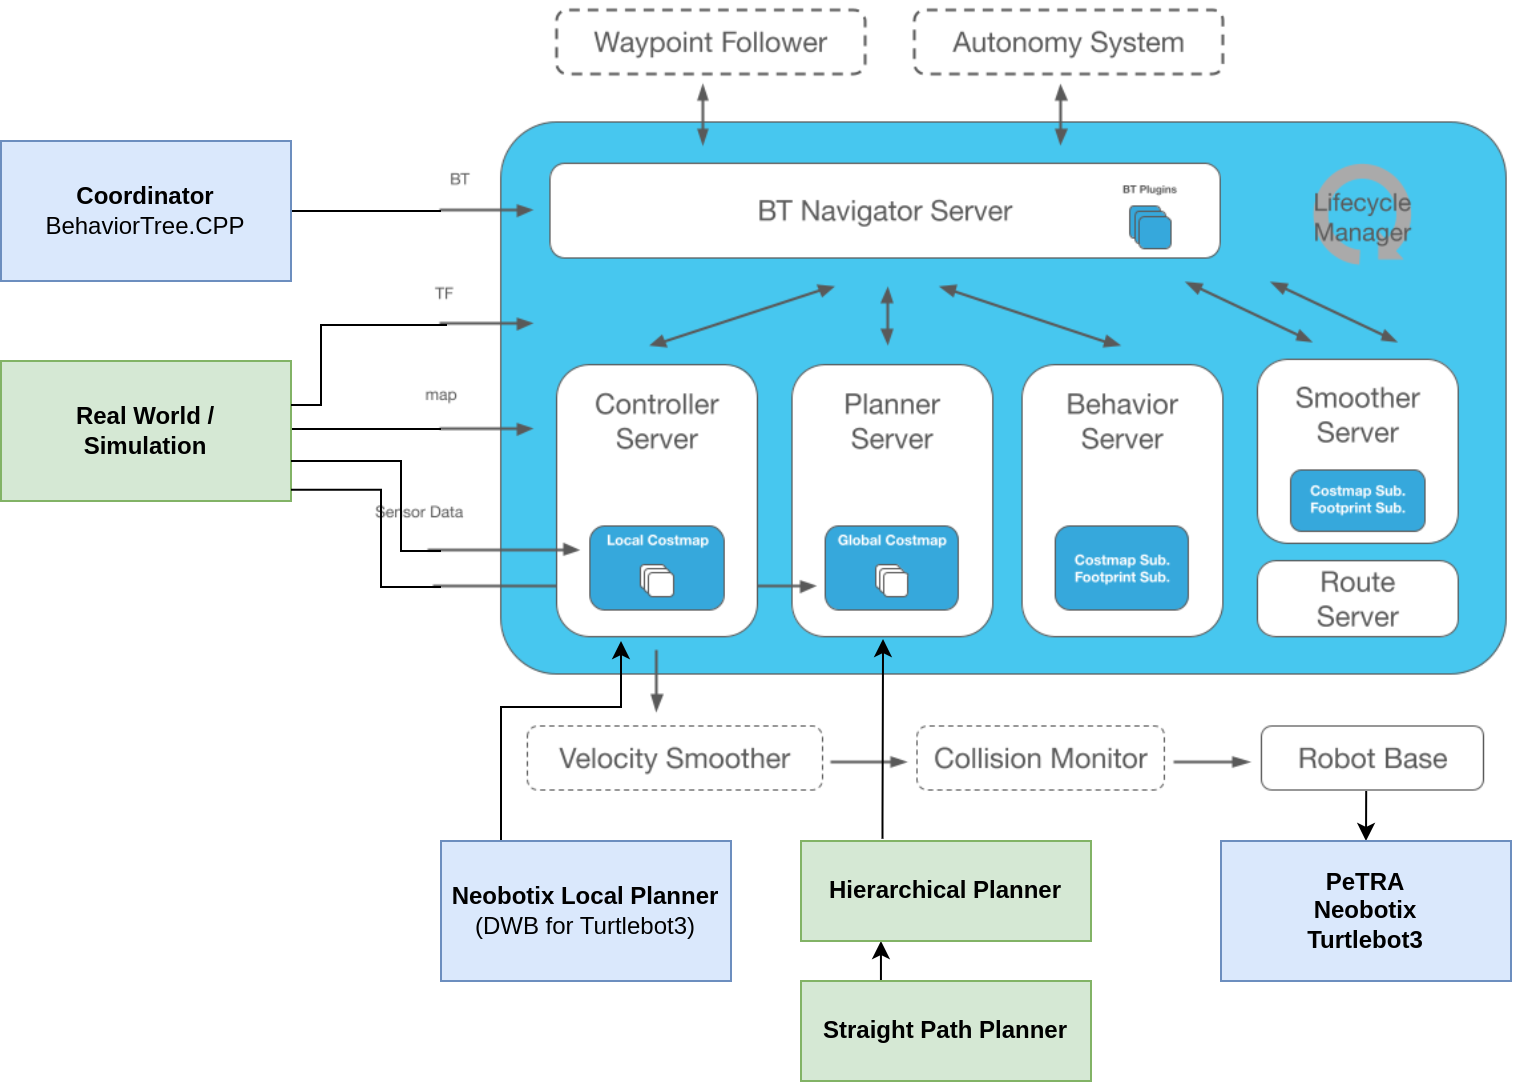
\includegraphics[width=\textwidth]{figures/40_concept/concept_nav2.png}
    \caption[The architecture of the Nav2 stack extended with custom nodes for hierarchical planning and (simulated) hardware]{The architecture of the Nav2 stack was extended with custom nodes for hierarchical planning and (simulated) hardware. Blue components were taken from the community, green components were developed in this work.}
    \label{fig:concept_nav2}
\end{figure}

The modular server-client architecture for Controller, Planner, Behavior and Smoother allows to swap the default implementations. In this case, the Controller, also known as the local planner, is used from the Neobotix MPO\_500 robot. This robot was used as a development platform for PeTRA and its planners provided better accuracy and customizability than the default \gls{dwa} controller. For this reason the Neobotix local planner \cite{pradheep_krishna_neobotixneo_local_planner2_2021} is used for PeTRA as well as for the MPO\_500 in real world and simulation. Only for testing with the Turtlebot3 the DWB controller was used, which is a further development of the DWA controller. As global planner the previously described Hierarchical Planner is used. For roadmap generation this planner plugin uses the \gls{ilir} straight path planner. The inputs to this navigation system come from the robot hardware, where it does not matter whether the sensor information is retrieved from the real world or from the gazebo simulation. The high-level task coordination is done by the Coordinator node, which uses the BT framework BehaviorTree.CPP \cite{auryn_robotics_behaviortreecpp_2023}. Figure \ref{fig:concept_uml} describes the interactions between these components in more detail. The diagram is loosely based on the \gls{uml} representation of these classes.

\begin{figure}[h]
    \centering
    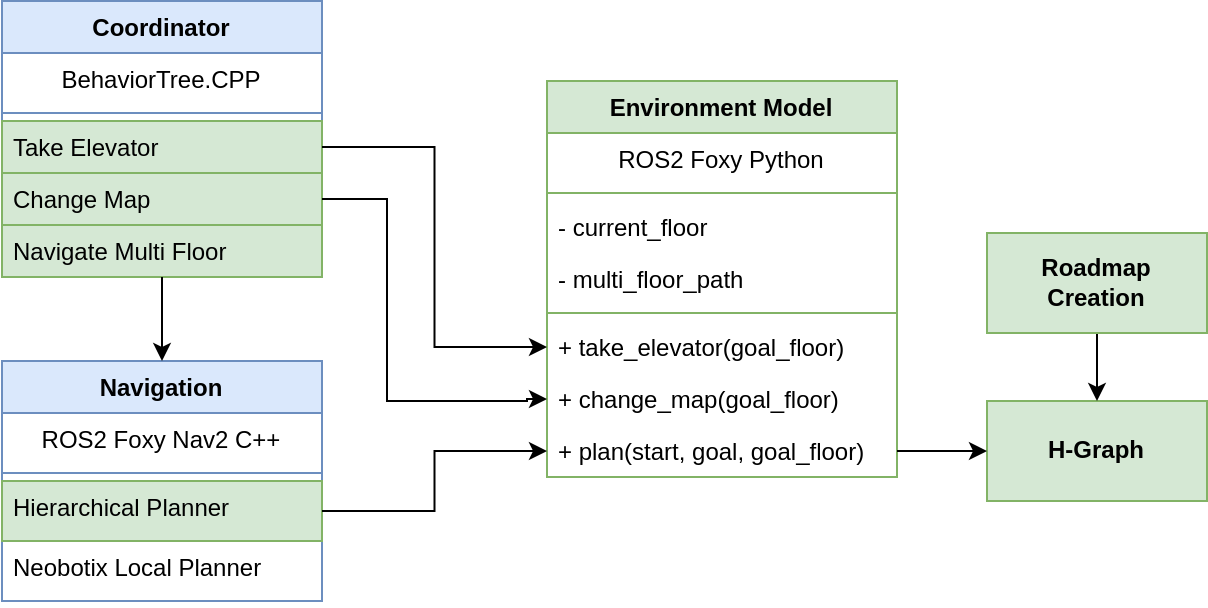
\includegraphics[width=0.75\textwidth]{figures/40_concept/concept_uml.png}
    \caption[Interactions between the custom components for multi-floor navigation]{Interactions between the custom components for multi-floor navigation. Blue components were taken from the community, green components were developed in this work.}
    \label{fig:concept_uml}
\end{figure}

The core component for storing information about the environment and thus enabling multi-floor navigation is the Environment Model. This ROS 2 node stores the current floor, holds the H-Graph with the gridmaps for all other floors, and executes floor and map changes by updating the appropriate information. The process for a multi-floor navigation task is as follows: First, the H-Graph of the environment is created with the precomputed roadmap from the ILIR planner and stored by the Environment Model. A single planning request is triggered by the Coordinator's current BT through the Navigate Multi Floor action. This is handled by the default action server of the \gls{nav_2} stack. The loaded custom planner plugin for the Hierarchical Planner sends a planning request to the H-Graph of the Environment Model. There, hierarchical planning is performed, taking into account additional information such as the current floor. This is important because the path returned by the Environment Model contains only the path on the current floor that can be executed by the \gls{nav_2} stack with the currently loaded map. All other paths on different floors and hierarchy levels are stored in the private variable multi\_floor\_path. It is necessary to store this information even though only the path on the current floor is executed. It is used to know which gridmap to load next and which elevator and floor number to call to reach the final destination. As soon as the robot reaches the elevator on the current map, the BT triggers the Take Elevator and then the Map Change actions. For the latter, the Environment Model loads the new gridmap and updates the internal state information. Take Elevator is only used by the Environment Model to provide information about the next destination floor, such as the floor number, the exact waiting position in front of the elevator, and the location of the control panel inside the elevator. This is not the complete action for Take Elevator, as the BT then executes the necessary actions to perform the actual operation of calling the elevator, selecting the floor, entering the elevator, and exiting at the target floor. For detailed information on the BT that coordinates these behaviors, see Chapter \ref{sec:multi_floor_behavior_trees}. In the simplest case in the hospital simulation, this action simply teleports the simulation's robot model to the appropriate position in front of the elevator on the target floor. After the robot reaches the target floor, the Coordinator again triggers a Navigate Multi Floor action, but this time it gets the path on the new floor from the Environment Model.

The last problem to be solved from the list at the beginning of this chapter is the interaction with the infrastructure. As mentioned before, it is the Coordinator's responsibility to trigger all the necessary actions to perform an elevator transition. However, the specific implementation of this BT depends very much on the available infrastructure, the degree of automation and the capabilities of the robot itself. The same applies to all connections at the same level, such as doors between rooms. These can also be very different: from doors with handles, to a button for automatic opening, to a revolving door. As this work is part of the PeTRA research project with several hospitals as partners, the use case focuses on their needs. The infrastructure of these hospitals is not up to date and has a very low level of automation and WiFi coverage. Considering this, some obstacles like closed doors with handles are out of scope for this work. In an ideal environment for mobile service robots, this infrastructure would provide WiFi interfaces to automatically trigger a door to open or an elevator to travel to the specified floor. In most current environments, this is not the case, and much research needs to be done in this area to establish a common interface protocol that works safely and securely with service robots. One attempt to unify these interfaces is the open source project Open-RMF \cite{openrobotics_open-rmf_2023} from Open Robotics. The use case for this work considers the capabilities of the PeTRA robot. With its integrated 5 \gls{dof} arm, PeTRA can also perform material transport of small custom boxes. This arm is also used to call the elevator and push the button for the target floor. The concept and implementation of this elevator operation is not part of this work, but is addressed in a related project. The infrastructure interaction concept of this work is limited to providing all necessary information and processes to trigger and execute this subtask as part of the overall multi-floor navigation.